\subsection{Versuchsaufbau}
\label{sec:Versuchsaufbau}
\subsubsection{Aufbau zur Ablenkung durch ein elektrisches Feld}
Der Aufbau zur Untersuchung der Proportionalität zwischen der Leuchtfleckverschiebung $D$ und
der Ablenkspannung $U_{\mathrm{d}}$ ist in Abbildung \ref{fig:verschiebungefeld} dargestellt.
\begin{figure}
  \centering
  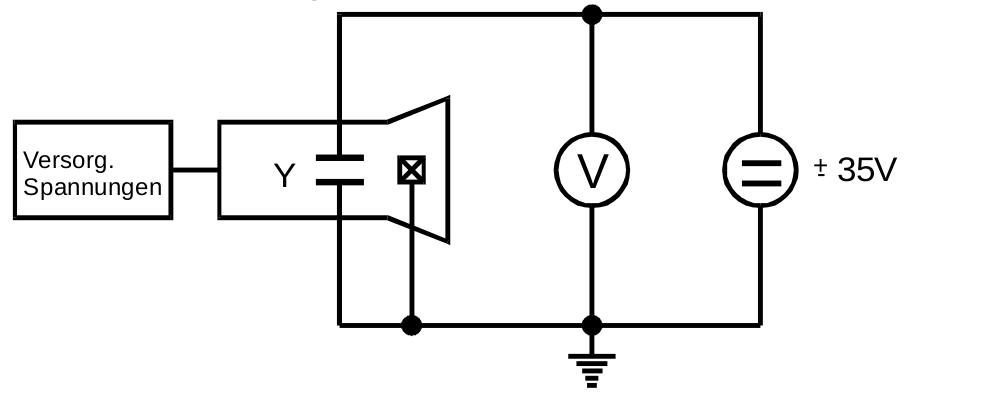
\includegraphics[width=0.8\textwidth]{Messdaten/schaltungefeld.png}
  \caption{Prinzipieller Aufbau zur Untersuchung der Proportionalität zwischen Leuchtfleckverschiebung $D$ und der Ablenkspannung $U_\mathrm{d}$.}
  \label{fig:verschiebungefeld}
\end{figure}
Dieser besteht aus der Kathodenstrahlröhre und einem Voltmeter zur Spannungsmessung. Für den
Schirm am Ende der Kathodenstrahlröhre soll das Y-System eingestellt werden, sodass die
Verschiebung nur in y-Richtung gemessen wird. Es ist darauf zu achten, dass eine Platte
der Ablenksysteme geerdet ist.
\begin{figure}
  \centering
  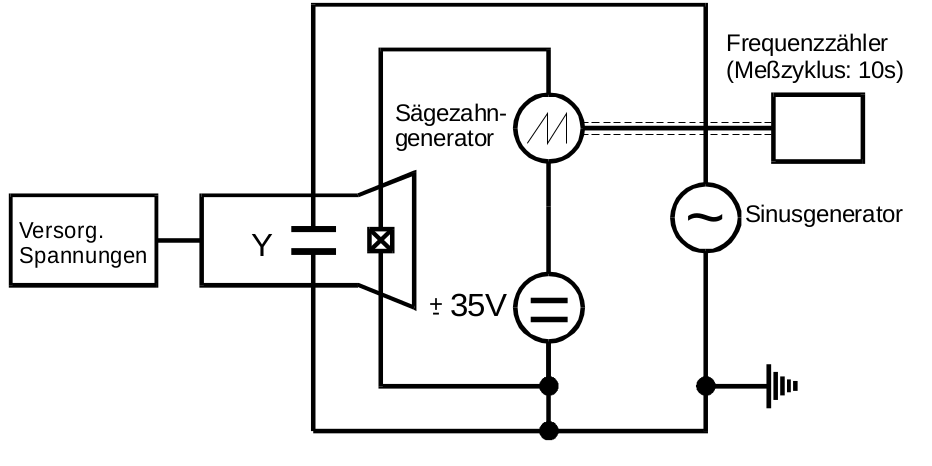
\includegraphics[width=0.8\textwidth]{Messdaten/oszi.png}
  \caption{Prinzipieller Aufbau eines Kathodenstrahl-Oszilloskop.}
  \label{fig:oszillo}
\end{figure}
Ein Kathodenstrahl-Oszillograph kann mit einem Aufbau wie in Abbildung \ref{fig:oszillo}
realisiert werden. Hierbei wird im Vergleich zum vorherigen Aufbau nur ein Sinusgenerator für
die Spannungsversorgung der in y-Richtung ablenkenden Platten und ein Sägezahngenerator
für die Spannungsversorgung der in x-Richtung ablenkenden Platten hinzugefügt.
Da bei dem Messvorgang die Sägezahnfrequenz bestimmt werden soll, wird außerdem ein
Frequenzzähler verwendet.

\subsubsection{Aufbau zur Ablenkung durch ein magnetisches Feld}
Für die Messung der Leuchtfleckverschiebung durch ein magnetisches Feld wird der Aufbau wie
in \ref{fig:verschiebungefeld} verwendet. Zusätzlich wird ein Magnetfeld in Form eines
Helmholtz-Spulenpaares senkrecht zur Kathodenstrahlröhre erzeugt. Der Spulenstrom kann manuell
reguliert werden.
Zur Bestimmung der Richtung des Erdmagnetfeldes wird ein Deklinatorium-Inklinatorium
verwendet.
